\documentclass[aspectratio=169,10pt]{beamer}
\usetheme{Madrid}
\usecolortheme{seahorse}
\usefonttheme{professionalfonts}

\usepackage[utf8]{inputenc}
\usepackage[T1]{fontenc}
\usepackage{amsmath,amssymb,amsthm}
\usepackage{graphicx}
\usepackage{xcolor}
\usepackage{listings}
\usepackage{booktabs}
\usepackage{array}

\graphicspath{{figures/}}

% ---------------------------------------------------------------------
% listings style
% ---------------------------------------------------------------------
\lstset{
  language=Python,
  basicstyle=\ttfamily\scriptsize,
  numbers=left,
  numberstyle=\tiny\color{gray},
  frame=single,
  backgroundcolor=\color{gray!7},
  commentstyle=\color{green!50!black}\itshape,
  keywordstyle=\color{blue}\bfseries,
  stringstyle=\color{purple},
  showstringspaces=false,
  breaklines=true,
  tabsize=2
}

% ---------------------------------------------------------------------
% beamer cosmetics
% ---------------------------------------------------------------------
\setbeamertemplate{footline}[frame number]
\setbeamertemplate{navigation symbols}{}

% ---------------------------------------------------------------------
% title data
% ---------------------------------------------------------------------
\title[UAI -- Ch.2.4]{An Introduction to Universal Artificial Intelligence}
\subtitle{Chapter 2.4: Bayesian Probability Theory}
\author{Based on Hutter, Quarel \& Catt (2024)}
\date{}

\begin{document}

% =======================================================================
\begin{frame}
  \titlepage
\end{frame}

\begin{frame}{Outline}
  \tableofcontents
\end{frame}

% =======================================================================
\section{Motivation: Why Not Just Use MLE?}

\begin{frame}{From frequentist statistics to Bayesian statistics}
  The previous section (2.3) covered \emph{frequentist} statistics: powerful
  and elegant estimators such as the maximum likelihood estimator (MLE), but
  with no single unifying principle, and with the uncertainty about the true
  probability measure handled only indirectly (e.g.\ via confidence
  intervals, which are routinely misinterpreted).

  \begin{block}{The Bayesian idea}
    In Bayesian statistics, uncertainty about the underlying probability
    measure is itself modelled \emph{by probabilities}. Starting from a
    \emph{prior} $w_\theta$ (belief $=$ epistemic probability) over the
    unknown parameter $\theta\in\Theta$, Bayes' rule is the general and
    optimal learning rule that uniquely determines how to update the prior to
    a \emph{posterior} belief probability once new data (evidence) arrives.
  \end{block}

  We first recall Bayes' rule for events, then specialise it to a simple
  binary i.i.d.\ setting, which leads to the famous \emph{Laplace rule}.
  Later chapters extend this machinery to much larger, in fact
  \emph{universal}, model classes and priors (Solomonoff induction, AIXI).
\end{frame}

\begin{frame}{Example 2.4.1: Estimating the lottery-winning probability}
  \begin{block}{Setup}
    Consider buying your very first lottery ticket, and you get lucky and win
    on the first try. Let $\theta$ be the true (unknown) probability of
    winning with a single ticket.
  \end{block}

  Lacking any prior knowledge about lotteries, the maximum likelihood
  estimator (MLE) would conclude from this single data point ``win'' that
  $\hat\theta_{\mathrm{MLE}}=1$: i.e.\ that you are \emph{guaranteed} to win
  the lottery every single time you play.

  \vspace{0.3cm}
  \textbf{Why this is implausible.} We already possess strong prior knowledge
  about lotteries: out of the many tickets sold, only a few are winners, so
  winning should be a very rare event. A frequentist estimator that ignores
  this prior knowledge and treats every parameter value as equally
  consistent with the data can produce absurdly overconfident conclusions
  when the sample size is tiny.

  \vspace{0.3cm}
  \textbf{Coin-flip analogy.} If we are estimating the bias $\theta$ (theta)
  of a coin, we expect an ordinary coin to have $\theta\approx\frac12$. After
  observing the coin land at least once on heads and at least once on tails,
  we can already rule out the extreme options $\theta=0$ or $\theta=1$ --
  something the naive MLE cannot do robustly from very little data.
\end{frame}

\begin{frame}{Fixing the problem: priors and posteriors}
  \begin{itemize}
    \item A frequentist approach \emph{can} converge to the truth in the
      limit of a lot of data, but for \emph{small} amounts of data we should
      also incorporate current prior domain knowledge about the parameter of
      interest into the estimation procedure.
    \item The distribution over the set of parameters given the domain
      knowledge, \emph{before} seeing any data, is called the \emph{prior}.
    \item \textbf{Bayes' Rule} gives a systematic method for turning the
      prior into a new distribution after having received the data, called
      the \emph{posterior}.
  \end{itemize}

  \begin{block}{Roadmap for this section}
    \begin{enumerate}
      \item \textbf{2.4.1} Bayes' Theorem for events, and the different
        interpretations of ``probability.''
      \item \textbf{2.4.2} Bayes estimation and prediction for a parameter
        $\theta$: joint distribution, mixture/evidence, posterior,
        predictive distribution.
      \item \textbf{2.4.3} The Laplace rule: a fully worked binary i.i.d.\
        example, the Beta distribution, the Jeffreys/KT prior, and the
        mean/variance of the posterior.
    \end{enumerate}
  \end{block}
\end{frame}

% =======================================================================
\section{2.4.1 Bayes' Theorem}

\begin{frame}{Bayes' celebrated theorem}
  Bayes' theorem allows the conditional probability $\mathrm P(A\mid B)$ to
  be computed in terms of $\mathrm P(A)$, $\mathrm P(B)$, and
  $\mathrm P(B\mid A)$.

  \begin{block}{Theorem 2.4.2 (Bayes' theorem)}
    Let $D\subseteq\Omega$ be an event with $\mathrm P(D)>0$ and
    $(H_i)_{i\in I}$ be a countable partition of $\Omega$ (i.e.\
    $\forall i\ne j: H_i\cap H_j=\varnothing$ and
    $\dot\bigcup_i H_i=\Omega$). Then
    \[
      \mathrm P(H_i\mid D) \;=\; \frac{\mathrm P(D\mid H_i)\,\mathrm P(H_i)}{\mathrm P(D)}
      \;=\; \frac{\mathrm P(D\mid H_i)\,\mathrm P(H_i)}{\sum_{j\in I}\mathrm P(D\mid H_j)\,\mathrm P(H_j)}.
    \]
  \end{block}

  \textbf{Plain-English reading of every symbol.} $\Omega$ is the whole
  sample space (``everything that could happen''); the sets $H_i$ are
  mutually exclusive \emph{hypotheses} that together cover every
  possibility (a \emph{partition}); $D$ is the observed \emph{data} or
  \emph{evidence}; $\mathrm P(H_i)$ is the \emph{prior} belief in hypothesis
  $H_i$ (before seeing $D$); $\mathrm P(D\mid H_i)$ is the \emph{likelihood}
  of the data under hypothesis $H_i$; and $\mathrm P(H_i\mid D)$ is the
  \emph{posterior} belief in $H_i$ after observing $D$. The key quantity
  $\mathrm P(D)=\sum_{j}\mathrm P(D\mid H_j)\mathrm P(H_j)$ is called the
  \emph{Bayesian evidence}, the \emph{marginal distribution}, or the
  \emph{mixture distribution}.
\end{frame}

\begin{frame}[allowframebreaks]{Interpretation: what does Bayes' theorem give us?}
  The intuition behind Bayes' theorem is that it provides a method of
  \emph{updating} (belief) probabilities based on evidence. Say $H_1$ is the
  hypothesis that a person has a particular disease, and $H_0$ that they do
  not. Before any clinical test, the doctor holds a subjective belief
  $\mathrm P(H_i)$, e.g.\ based on symptoms and demographics. After the test
  result $D$ arrives, this belief updates to $\mathrm P(H_i\mid D)$, which
  may increase or decrease the confidence in $H_i$ depending on whether $D$
  is evidence for or against it.

  \textbf{Mathematically}, the Bayesian ``sample'' space $\Omega$ is a
  product of a data (frequentist) sample space $\Omega_D$ and a hypothesis
  space $\Omega_H$. A hypothesis $H_i$ is an event of the form
  $\Omega_D\times\{\tilde H_i\}\subset\Omega$; an observation $D$ is an
  event of the form $\tilde D\times\Omega_H\subset\Omega$. Usually
  $\tilde H_i\in\Omega_H$ and $\tilde D\subset\Omega_D$ are what get
  specified, with the tilde dropped and the lifting to the product space
  implicit.

  Different people can hold different confidences in the same events: the
  patient and the doctor generally have different priors $\mathrm P(H_i)$
  (the doctor has more experience judging base rates, the patient's belief
  may be driven more by fear or wishful thinking), and hence, even after
  both learn about $D$, they will typically hold different posteriors too.

  \framebreak

  \textbf{Four interpretations of ``probability.''}
  \begin{itemize}
    \item \textbf{Frequentist:} Probabilities are the relative frequency of
      an event occurring. In a sequence of $n$ i.i.d.\ trials, if an event
      occurs $k(n)$ times, its relative frequency is $k(n)/n$, and the
      probability of the event is defined as the limit
      $\lim_{n\to\infty}k(n)/n$. Frequentists model $\mathrm P(D\mid H_i)$
      but assign \emph{neither} a prior nor a posterior probability to
      $H_i$.
    \item \textbf{Objectivist:} Probabilities are real aspects of the world
      (``true'' probabilities). Outcomes are not deterministic but involve
      chaotic or random physical processes. They should be consistent with
      limiting frequencies for i.i.d.\ experiments, but are not limited to
      that case -- e.g.\ the probability of a volcanic eruption in a specific
      century is a unique, non-i.i.d., stochastic-process probability.
    \item \textbf{Subjectivist:} Probabilities are merely subjective, and
      represent a \emph{particular individual's} confidence or degree of
      belief, called \emph{epistemic} probability. Subjective probabilities
      depend on who holds them (doctor vs.\ patient) and on what extra
      information is available.
    \item \textbf{Bayesian:} A Bayesian assigns a prior probability over
      $H_i$ \emph{and} uses a (frequentist) likelihood model
      $\mathrm P(D\mid H_i)$ to update the prior $\mathrm P(H_i)$ to a
      posterior $\mathrm P(H_i\mid D)$ after observing evidence $D$. The
      prior may be \emph{subjective} (e.g.\ from expert elicitation) or
      \emph{objective} (like the Jeffreys prior below), or \emph{universal}
      (Section 3.7) -- though this trichotomy is a gross over-simplification.
  \end{itemize}

  Remarkably, \emph{all} of these interpretations satisfy the very same
  Kolmogorov axioms of probability -- they differ only in what probability
  is taken to \emph{mean}, not in the mathematics governing it.
\end{frame}

\begin{frame}{Example 2.4.3: Blood type testing}
  \begin{block}{Setup}
    Blood type O-negative ($O^-$) can be donated to anyone, and $7\%$ of the
    population has it: $\mathrm P(H^-)=0.07$ where $H^-$ is ``Person $A$ has
    blood type $O^-$'' and $H^+=\overline{H^-}$. A test is $95\%$ accurate:
    if you truly have (do not have) $O^-$ blood, it returns a false
    negative (positive) with probability $5\%$. The test on a random person
    comes back \emph{positive} for $O^-$. How confident should we be that
    this person \emph{actually} has $O^-$ blood?
  \end{block}

  Let $D^-$ be the event ``the test says $O^-$.'' The likelihoods are
  $\mathrm P(D^-\mid H^-)=\mathrm P(D^+\mid H^+)=0.95$ (correct results) and
  $\mathrm P(D^-\mid H^+)=\mathrm P(D^+\mid H^-)=0.05$ (errors). Applying
  Bayes' Theorem 2.4.2 with hypothesis space $\Omega_H=\{H^-,H^+\}$:
  \[
    \mathrm P(H^-\mid D^-) \;=\; \frac{\mathrm P(D^-\mid H^-)\,\mathrm P(H^-)}
        {\mathrm P(D^-\mid H^-)\,\mathrm P(H^-) + \mathrm P(D^-\mid H^+)\,\mathrm P(H^+)}
        \;=\; \frac{0.95\times 0.07}{0.95\times 0.07 + 0.05\times 0.93}
        \;\approx\; 59\%.
  \]
  Every symbol: the numerator is (probability test is correct)$\times$(prior
  probability of actually having $O^-$); the denominator additionally sums
  in the probability that the test falsely reports $O^-$ for an $H^+$ person.
\end{frame}

\begin{frame}{Blood type testing: why the answer feels counter-intuitive}
  A symmetric calculation for a \emph{negative} test result gives
  \[
    \mathrm P(H^-\mid D^+) \;=\; \frac{\mathrm P(D^+\mid H^-)\,\mathrm P(H^-)}
        {\mathrm P(D^+\mid H^-)\,\mathrm P(H^-) + \mathrm P(D^+\mid H^+)\,\mathrm P(H^+)}
        \;=\; \frac{0.05\times 0.07}{0.05\times 0.07 + 0.95\times 0.93}
        \;\approx\; 0.4\%.
  \]

  \textbf{Interpretation.} Despite the test having a relatively high success
  probability ($95\%$), the probability of \emph{actually} having $O^-$
  blood given a positive test is only $\approx 59\%$. This is due to the
  small \emph{base rate} (prior probability) of $O^-$ blood: since the
  probability of a false positive ($5\%$) and the probability of truly
  having $O^-$ blood ($7\%$) are of similar magnitude, roughly half the
  positive test results come from the test being wrong and half from
  genuinely $O^-$ patients. Conversely, since non-$O^-$ blood is so common,
  a \emph{negative} result is very strong evidence of not having $O^-$
  blood, since that would require \emph{both} an unlikely event (having
  $O^-$) \emph{and} the reliable test failing.

  \begin{block}{Take-away}
    Always weigh the likelihood ratio against the \emph{prior odds}
    $\mathrm P(H^-)/\mathrm P(H^+)$ -- an accurate test can still leave you
    quite uncertain when the condition being tested for is rare.
  \end{block}
\end{frame}

\begin{frame}[fragile]{Python: verifying the blood-type posterior}
  \begin{lstlisting}
# Exact re-derivation of Example 2.4.3 by direct computation.
P_Hminus = 0.07          # prior P(H^-):  7% of population is O-negative
P_Hplus  = 1 - P_Hminus  # prior P(H^+)

# Likelihoods: test is 95% accurate either way
P_Dminus_given_Hminus = 0.95   # P(D^-|H^-): true positive rate
P_Dminus_given_Hplus  = 0.05   # P(D^-|H^+): false positive rate
P_Dplus_given_Hminus  = 0.05   # P(D^+|H^-): false negative rate
P_Dplus_given_Hplus   = 0.95   # P(D^+|H^+): true negative rate

# Bayes' theorem: posterior = likelihood * prior / evidence
num_pos = P_Dminus_given_Hminus * P_Hminus
den_pos = num_pos + P_Dminus_given_Hplus * P_Hplus
post_Hminus_given_Dminus = num_pos / den_pos

num_neg = P_Dplus_given_Hminus * P_Hminus
den_neg = num_neg + P_Dplus_given_Hplus * P_Hplus
post_Hminus_given_Dplus = num_neg / den_neg

print(f"P(H- | test positive) = {post_Hminus_given_Dminus:.4f}")  # ~0.5891
print(f"P(H- | test negative) = {post_Hminus_given_Dplus:.4f}")  # ~0.0038
  \end{lstlisting}
  Running this script reproduces exactly $\approx 59\%$ and $\approx 0.4\%$,
  confirming the hand calculation above and showing how directly Bayes'
  theorem translates into three lines of arithmetic.
\end{frame}

% =======================================================================
\section{2.4.2 Bayes Estimation and Prediction}

\begin{frame}{From events to parameters: modelling uncertainty about $\theta$}
  We now express our belief over plausible and implausible values of
  $\theta\in\Theta$ as a \emph{density function} $w(\theta)$, called the
  \emph{prior}.

  \begin{itemize}
    \item In \emph{frequentist} statistics, $\theta$ is \textbf{not} a
      random variable: the true value of the parameter (e.g.\ the bias of a
      coin) is a fixed, though unknown, constant. Frequentists \emph{can}
      express uncertainty in $\theta$ (e.g.\ via confidence intervals), but
      the interpretation is convoluted and often confused even by
      statisticians.
    \item \emph{Bayesians} instead model uncertainty about $\theta$ in
      exactly the same way as for observations $X$: they \emph{treat $\theta$
      as a random variable} and assign a (subjective) prior distribution
      $w(\theta)$ over it, encoding our prior beliefs about the relative
      plausibility of values of $\theta\in\Theta$.
  \end{itemize}

  This requires enlarging the sample space to
  $\Omega''=\Omega\times\Omega'$ to accommodate $\theta$, where $X(\omega)$
  becomes $X(\omega'')$. Typically $\Omega'=\Theta$, and with some abuse of
  notation $\theta(\omega')=\omega'$. Mathematically $\theta$ is now a random
  variable and $\Theta$ is part of the sample space -- even though most
  Bayesians would \emph{not} literally interpret $\theta$ as ``random'' or
  ``sampled''; the clash in nomenclature is more than compensated by the
  mathematical convenience this unified treatment offers.
\end{frame}

\begin{frame}{Joint, marginal, and posterior distributions}
  The probability distribution $p_X(x;\theta)$ for observed random variables
  $X$ can be viewed as a conditional distribution on $X$ given $\theta$,
  formalised by defining the \emph{joint} distribution
  \[
    p(x,\theta) \;:=\; p_X(x;\theta)\,w(\theta).
  \]
  Every symbol: $x$ is a possible value of the data, $\theta$ (theta) is the
  unknown parameter, $p_X(x;\theta)$ is the model's likelihood of $x$ given
  $\theta$, and $w(\theta)$ is the prior density over $\theta$. Then
  $p(x\mid\theta)\equiv p(x,\theta)/w(\theta)=p_X(x;\theta)$ whenever
  $w(\theta)>0$.

  \begin{block}{The mixture (marginal / Bayesian-evidence) distribution}
    \[
      p(x_1,\ldots,x_n) \;=\; \int_\Theta p(x_1,\ldots,x_n\mid\vartheta)\,w(\vartheta)\,d\vartheta.
    \]
  \end{block}
  This is the probability of the data \emph{averaged over all values of}
  $\theta$, weighted by the prior; $\vartheta$ (a variant form of theta) is
  just the integration (dummy) variable ranging over $\Theta$. This
  quantity is central to Bayesian statistics: \textbf{as a rule of thumb, if
  the mixture can be efficiently computed, then everything else of interest
  can be efficiently computed too.}
\end{frame}

\begin{frame}{Bayes' rule for parameters: prior $\to$ posterior}
  A continuous version of Bayes' Theorem 2.4.2 updates the prior belief
  about $\theta$ with observations $x_1,\ldots,x_n$ to arrive at the
  \emph{posterior} belief distribution
  \begin{block}{Posterior distribution}
    \[
      w(\theta\mid x_1,\ldots,x_n) \;=\; \frac{p(x_1,\ldots,x_n\mid\theta)\,w(\theta)}{p(x_1,\ldots,x_n)}.
    \]
  \end{block}
  Every symbol: the numerator multiplies the \emph{likelihood} of the
  observed data given $\theta$ by the \emph{prior} density at $\theta$; the
  denominator is the mixture distribution (evidence) from the previous
  slide, which normalises the result back into a valid density over
  $\theta$. This posterior combines two sources of information: our prior
  beliefs about what $\theta$ should be, and any evidence provided by the
  observed data. Bayes' rule \emph{uniquely} determines the posterior given
  a prior -- i.e.\ it is the one and only consistent way to update beliefs
  based on evidence.
\end{frame}

\begin{frame}{Predicting new data from the posterior}
  Often estimating $\theta$ is merely a means to an end: what we ultimately
  want is to make \emph{predictions}.

  \begin{block}{Predictive distribution (2.4.4)}
    \[
      p(x_{n+1}\mid x_1,\ldots,x_n) \;=\; \int_\Theta p(x_{n+1}\mid\vartheta)\,w(\vartheta\mid x_1,\ldots,x_n)\,d\vartheta
      \;=\; \frac{p(x_1,\ldots,x_{n+1})}{p(x_1,\ldots,x_n)}.
    \]
  \end{block}
  Every symbol: $x_{n+1}$ is the next, not-yet-observed data point;
  $w(\vartheta\mid x_1,\ldots,x_n)$ is the posterior density over $\theta$
  from the previous slide; and the integral averages the model's
  prediction $p(x_{n+1}\mid\vartheta)$ over every possible value of
  $\vartheta$, weighted by how plausible the posterior currently considers
  that value. The predictive distribution therefore \emph{averages the
  model's prediction over the posterior uncertainty in $\theta$}, rather
  than committing to a single point estimate of $\theta$ and predicting
  from that alone -- this is what makes Bayesian prediction naturally
  ``humble'' about parameter uncertainty.
\end{frame}

% =======================================================================
\section{2.4.3 The Laplace Rule}

\begin{frame}{Setting up the running example: a biased coin}
  Section 2.4.2 explains \emph{how} to incorporate a prior, but is agnostic
  about \emph{where the prior comes from}. In practice, the choice of prior
  can greatly affect the estimate when little data is available, though with
  enough data the posterior concentrates on the true parameter for
  ``sensible'' prior choices. Choosing a canonical prior over a
  \emph{function space} that respects Occam's razor is a major focus of
  later chapters of the book (universal priors); here we work out the
  simplest possible case fully.

  \begin{block}{Derivation setup}
    Suppose we have a biased coin governed by a Bernoulli process with
    unknown parameter $\theta$: we observe a sequence of coin flips
    $x_1,x_2,\ldots\sim\mathrm{Bern}(\theta)$, and would like to estimate
    $\theta$ from the sequence. Applying Bayes' Theorem 2.4.2 gives the
    posterior
    \[
      w(\theta\mid x_1,\ldots,x_n) \;=\; \frac{p(x_1,\ldots,x_n\mid\theta)\,w(\theta)}
        {\int_\Theta p(x_1,\ldots,x_n\mid\vartheta)\,w(\vartheta)\,d\vartheta}
      \;=\; \frac{w(\theta)\prod_{i=1}^n\mathrm{Bern}(x_i;\theta)}
        {\int_\Theta w(\vartheta)\prod_{i=1}^n\mathrm{Bern}(x_i;\vartheta)\,d\vartheta}.\quad(2.4.5)
    \]
  \end{block}
  Since $\mathrm{Bern}(x;\theta)=\theta^x(1-\theta)^{1-x}$, the product
  $\prod_{i=1}^n\mathrm{Bern}(x_i;\theta)=\theta^b(1-\theta)^a$, where $a$ is
  the number of zeros and $b$ the number of ones in $x_1,\ldots,x_n$.
\end{frame}

\begin{frame}{The Beta distribution}
  \begin{block}{Definition (2.4.6): the Beta distribution}
    \[
      \mathrm{Beta}(\theta;\alpha,\beta) \;=\; \frac{1}{B(\alpha,\beta)}\,\theta^{\alpha-1}(1-\theta)^{\beta-1},
      \qquad \text{where } B(\alpha,\beta)=\int_0^1\theta^{\alpha-1}(1-\theta)^{\beta-1}\,d\theta
    \]
    is the \emph{beta function}, and $\alpha$ (alpha), $\beta$ (beta) $>0$
    are the two shape parameters of the distribution.
  \end{block}

  If we have no prior information about the coin, choosing a
  \textbf{uniform} distribution over $[0,1]$ for our prior belief in
  $\theta$ is reasonable. This should \textbf{not} be interpreted as a
  ``lack of a prior belief'' -- it in fact expresses a prior belief of
  \emph{indifference}: every value in $[0,1]$ is deemed \emph{a priori} as
  likely as any other. Using $w(\theta)=1$ for $0\le\theta\le 1$ turns
  (2.4.5) into
  \[
    w(\theta\mid x_1,\ldots,x_n) \;=\; \frac{\theta^b(1-\theta)^a}{\int_0^1\vartheta^b(1-\vartheta)^a\,d\vartheta}
    \;=\; \frac{\theta^b(1-\theta)^a}{B(b+1,a+1)} \;=\; \mathrm{Beta}(\theta;b+1,a+1).
  \]
  So starting from a uniform prior, observing $b$ ones and $a$ zeros turns
  the prior into a $\mathrm{Beta}(b+1,a+1)$ posterior -- the counts $a,b$
  simply shift the Beta's shape parameters.
\end{frame}

\begin{frame}{Figure: the Beta density for various shape parameters}
  \begin{center}
    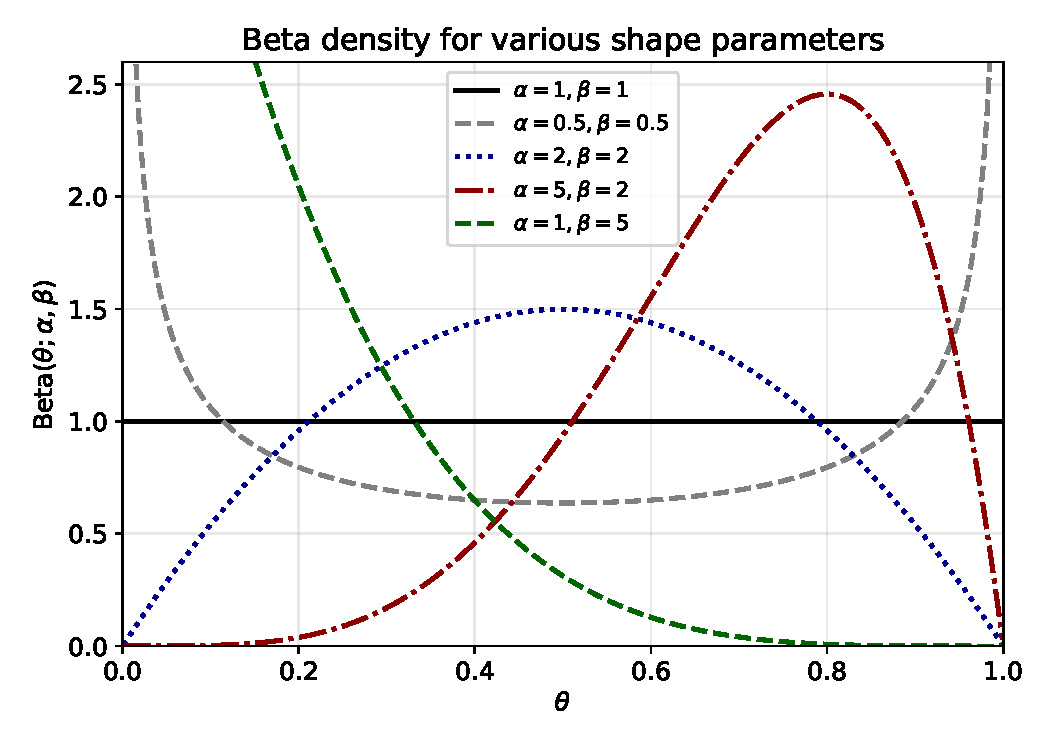
\includegraphics[height=4.3cm]{beta_family}
  \end{center}
  As $\alpha,\beta$ (alpha, beta) increase together and stay equal, the
  density concentrates more sharply around $\theta=\tfrac12$ (e.g.\ the
  dotted curve $\alpha=\beta=2$); when $\alpha\ne\beta$, the mode shifts
  towards $1$ or $0$ (e.g.\ the dash-dot curve $\alpha=5,\beta=2$ favours
  large $\theta$); and when $0<\alpha=\beta<1$ (dashed curve
  $\alpha=\beta=0.5$), probability mass piles up near the two extremes
  $0$ and $1$ instead of the middle.
\end{frame}

\begin{frame}{Figure: watching the posterior update, one bit at a time}
  \begin{center}
    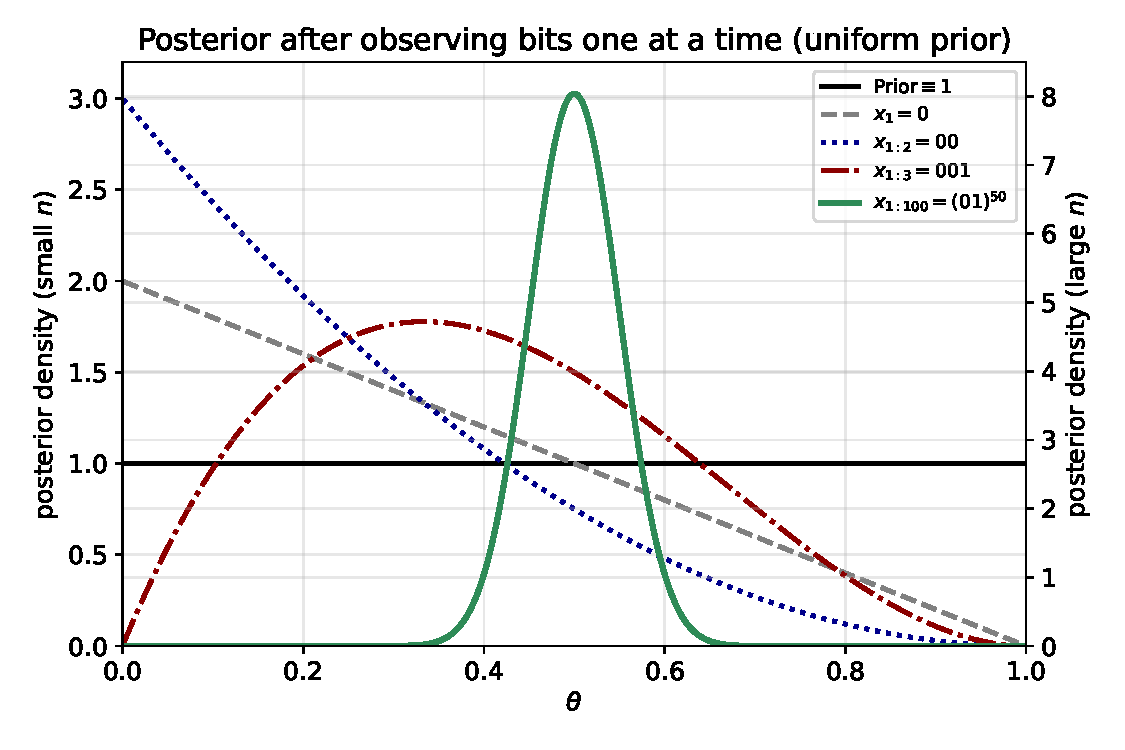
\includegraphics[height=4.3cm]{posterior_evolution}
  \end{center}
  Starting from a uniform prior ($n=0$, solid black line), the sequence
  $x_{1:3}=001$ is observed one bit at a time: the posterior shifts more
  probability mass towards \emph{smaller} $\theta$ after each $0$, then
  shifts back slightly once the $1$ is observed. The green curve
  (right-hand axis) shows the far sharper posterior after $100$ flips of
  alternating $0$s and $1$s, $x_{1:100}=(01)^{50}$: with far more data the
  posterior concentrates tightly around $\theta=\tfrac12$, exactly as
  expected for a fair coin.
\end{frame}

\begin{frame}{Predicting the next flip: deriving the Laplace rule}
  \small
  Given the posterior over $\theta$, we use the predictive distribution
  (2.4.4) to predict $x_{n+1}$. Since $X_{n+1}\sim\mathrm{Bern}(\theta)$
  means $\mathrm P(X_{n+1}=1\mid\theta)=\theta$,
  \[
    \mathrm P(X_{n+1}=1\mid x_1,\ldots,x_n) \;=\; \int_\Theta\theta\cdot\frac{\theta^b(1-\theta)^a}{B(b+1,a+1)}\,d\theta
    \;=\; \frac{\int_0^1\theta^{b+1}(1-\theta)^a\,d\theta}{B(b+1,a+1)}
    \;=\; \frac{B(b+2,a+1)}{B(b+1,a+1)}.
  \]
  \textbf{The Gamma function.} We simplify this using the \emph{Gamma
  function}
  \[
    \Gamma(k) \;:=\; \int_0^\infty x^{k-1}e^{-x}\,dx \quad (2.4.7),
  \]
  a continuous generalisation of the factorial, satisfying $\Gamma(k)=(k-1)!$
  for integer $k\ge 1$ and $\Gamma(z+1)=z\Gamma(z)$ for all $z\in\mathbb R$
  where $\Gamma(z)$ is defined. The Beta function satisfies, for any
  $a,b>0$,
  \[
    B(a,b) \;=\; B(b,a) \;=\; \int_0^1\theta^{b-1}(1-\theta)^{a-1}\,d\theta \;=\; \frac{\Gamma(a)\Gamma(b)}{\Gamma(a+b)}.
  \]
  Substituting this identity into $B(b+2,a+1)/B(b+1,a+1)$ and cancelling
  common Gamma-function factors (using $\Gamma(z+1)=z\Gamma(z)$
  repeatedly) yields, after simplification,
  \[
    \mathrm P(X_{n+1}=1\mid x_1,\ldots,x_n) \;=\; \frac{b+1}{a+b+2} \;=\; \frac{1}{n+2}\Bigl(1+\sum_{i=1}^n x_i\Bigr).
  \]
\end{frame}

\begin{frame}{Theorem 2.4.8: the Laplace rule}
  \begin{block}{Theorem 2.4.8 (Laplace rule)}
    For i.i.d.\ $X_i\sim\mathrm{Bern}(\theta)$ and a uniform prior
    $\theta\in[0,1]$,
    \[
      \mathrm P(X_{n+1}=1\mid X_1=x_1,\ldots,X_n=x_n) \;=\; \frac{k+1}{n+2},
      \qquad \text{where } k=\bigl|\{i\le n: x_i=1\}\bigr|=\sum_{i=1}^n x_i.
    \]
  \end{block}
  Every symbol: $n$ is the number of coin flips observed so far, $k$ is how
  many of them came up ``$1$,'' and the formula $(k+1)/(n+2)$ is the
  probability the estimator assigns to the \emph{next} flip being a $1$.
  This particular choice of (uniform) prior is called the \emph{indifference
  rule} or \emph{Laplace rule}, and the resulting estimator is the
  \emph{Laplace estimator}.

  \textbf{The sunrise problem.} If the sun has risen every day for all
  $1\le i\le n$ (so $x_i=1$ always), the Laplace rule gives the estimate
  $\frac{n+1}{n+2}$ that the sun will rise tomorrow -- a much less
  overconfident answer than the naive MLE's certainty of $1$, yet it still
  approaches $1$ as more days of evidence accumulate.
\end{frame}

\begin{frame}[fragile]{Python: Laplace rule in action}
  \begin{lstlisting}
def laplace_rule(sequence):
    """P(next flip = 1 | sequence), Theorem 2.4.8."""
    n = len(sequence)
    k = sum(sequence)          # number of ones observed
    return (k + 1) / (n + 2)

def mle(sequence):
    """Naive frequentist estimate: relative frequency of ones."""
    n = len(sequence)
    return None if n == 0 else sum(sequence) / n  # undefined @ n=0

# Example 2.4.1: a single winning lottery ticket
print("MLE after one win:    ", mle([1]))           # 1.0  (overconfident!)
print("Laplace after one win:", laplace_rule([1]))   # 0.667
# Sunrise problem: n=10000 days, sun rose every day
seq = [1] * 10000
print("MLE (sunrise, n=10000):    ", mle(seq))          # 1.0
print("Laplace (sunrise, n=10000):", laplace_rule(seq))  # 0.99980002
# Coin-flip sequence x_{1:3} = 0,0,1 from Figure 2.11
print("Laplace after 001:", laplace_rule([0, 0, 1]))  # 0.4
  \end{lstlisting}
  The Laplace rule never outputs exactly $0$ or $1$ for finite $n$, unlike
  the MLE, reflecting the Bayesian's built-in ``humility'' from the uniform
  prior.
\end{frame}

\begin{frame}{Figure: MLE versus the Laplace-rule estimate}
  \begin{center}
    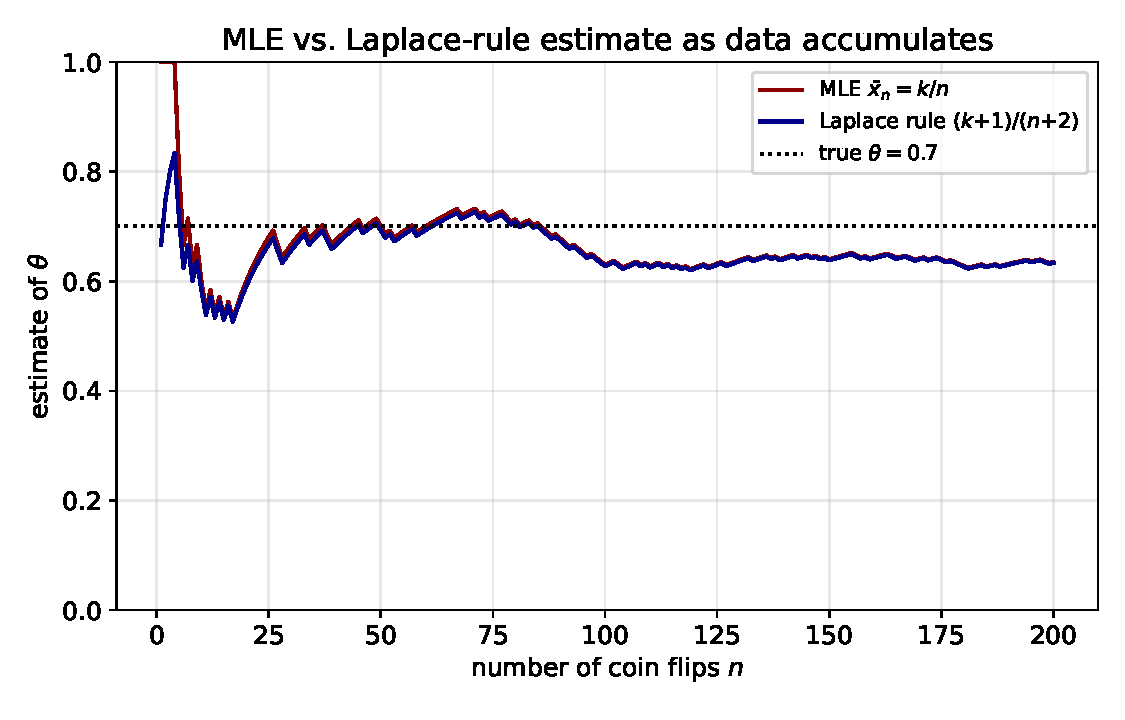
\includegraphics[height=4.3cm]{mle_vs_laplace}
  \end{center}
  A simulated sequence of $200$ coin flips with true bias $\theta=0.7$
  (dotted black line). The MLE (red) is noisier for small $n$ and can
  briefly touch $0$ or $1$; the Laplace-rule estimate (blue) is
  systematically pulled towards $\tfrac12$ for small $n$ (reflecting the
  uniform prior's ``pull'') but the two curves converge as $n$ grows, since
  the influence of any fixed prior vanishes as evidence accumulates.
\end{frame}

\begin{frame}{The general Beta prior}
  More generally, suppose we choose an arbitrary Beta distribution as our
  prior, $w(\theta)=\mathrm{Beta}(\theta;\alpha,\beta)$ for some
  $\alpha,\beta>0$ (the uniform prior is the special case
  $\alpha=\beta=1$, since $\mathrm{Beta}(\theta;1,1)=1$). Repeating the
  same calculation as before yields
  \begin{block}{Posterior and predictive distribution, general Beta prior}
    \[
      w(\theta\mid x_1,\ldots,x_n;\alpha,\beta) \;=\; \mathrm{Beta}(\theta;b+\alpha,a+\beta) \qquad (2.4.9)
    \]
    \[
      \mathrm P(X_{n+1}=1\mid x_1,\ldots,x_n;\alpha,\beta) \;=\; \frac{b+\beta}{a+b+\alpha+\beta}
      \;=\; \frac{\beta+\sum_{i=1}^n x_i}{n+\alpha+\beta}. \qquad (2.4.10)
    \]
  \end{block}
  \textbf{Pseudocounts.} The parameters $\alpha$ and $\beta$ can be thought
  of as \emph{hypothetical prior counts} of zeros and ones observed before
  the experiment even began (as if we had been told the outcome of some
  earlier, hypothetical experiment with the coin). Because they act like
  extra, imaginary observations that smooth out the rapid changes seen when
  very little real data is available, $\alpha$ and $\beta$ are called
  \emph{pseudocounts}, and they act as a \emph{regularizer}.
\end{frame}

\begin{frame}{Choosing $\alpha$ and $\beta$}
  If we have no information about whether a $0$ or a $1$ is more likely,
  \emph{a priori} it seems sensible to choose $\alpha=\beta$, eliminating
  one free parameter -- but we still need to pick the common value.

  \begin{itemize}
    \item $\alpha=\beta=1$: recovers the uniform (indifference) prior.
    \item $\alpha=\beta>1$: weights the prior more heavily towards
      $\theta\approx\tfrac12$, and is \emph{unlikely} to move towards the
      extremes $0$ or $1$ without a lot of contrary evidence. Appropriate
      when we have a strong prior belief that a coin is fair: with large
      $\alpha=\beta$, only a sufficiently large number of observations
      would persuade us the coin is unfair.
    \item $0<\alpha=\beta<1$: the opposite case -- a prior that is
      \emph{more} biased towards the extremes, expressing a prior
      assumption that the coin is likely to be unfair. In the extreme limit
      $\alpha=\beta\to 0$, the distribution degenerates into two point
      masses at $0$ and $1$, i.e.\ a prior assumption that the coin's
      outcome is fully \emph{deterministic}.
  \end{itemize}
\end{frame}

\begin{frame}{The Jeffreys prior}
  One principled approach for choosing $\alpha=\beta$ is to require the
  prior to be \emph{invariant under a change of coordinates} for the
  parameter $\theta$.

  \begin{block}{Definition 2.4.11 (Jeffreys prior)}
    The Jeffreys prior is a prior with density function proportional to the
    square root of the Fisher information:
    \[
      w(\theta) \;\propto\; \sqrt{\mathcal I(\theta)}.
    \]
  \end{block}
  Here $\mathcal I(\theta)$ (the calligraphic letter I) is the \emph{Fisher
  information} introduced in Section 2.3: it measures how much information
  each sample carries, on average, about $\theta$.

  We compute $\mathcal I(\theta)$ for $\mathrm{Bern}(x;\theta)$:
  \[
    \mathcal I(\theta) \;=\; -\mathbf E_\theta\Bigl[\tfrac{\partial^2}{\partial\theta^2}\ln\mathrm{Bern}(X;\theta)\Bigr]
    \;=\; \mathbf E_\theta\Bigl[\tfrac{X}{\theta^2}+\tfrac{1-X}{(1-\theta)^2}\Bigr]
    \;=\; \frac{\theta}{\theta^2}+\frac{1-\theta}{(1-\theta)^2} \;=\; \frac{1}{\theta(1-\theta)},
  \]
  using linearity of expectation and $\mathbf E_\theta[X]=\theta$. Hence
  $w(\theta)\propto 1/\sqrt{\theta(1-\theta)}$, which is exactly a Beta
  distribution with $\alpha=\beta=\tfrac12$.
\end{frame}

\begin{frame}{The KT estimator, and Jeffreys vs.\ uniform priors}
  \begin{columns}
    \begin{column}{0.5\textwidth}
      \begin{block}{The KT estimator}
        The estimator resulting from the Jeffreys prior
        $\mathrm{Beta}(\theta;\tfrac12,\tfrac12)$ is called the \emph{KT
        estimator} (Krichevsky--Trofimov), explored further in Section
        4.1. While this choice is invariant under reparametrisation and
        minimax optimal for a binary alphabet, other choices of $\alpha,
        \beta$ can perform better for large, non-binary alphabets.
      \end{block}
      From (2.4.10) with $\alpha=\beta=\tfrac12$, the KT predictive
      probability is
      \[
        \mathrm P(X_{n+1}=1\mid x_1,\ldots,x_n) = \frac{b+\tfrac12}{n+1}.
      \]
    \end{column}
    \begin{column}{0.5\textwidth}
      \begin{center}
        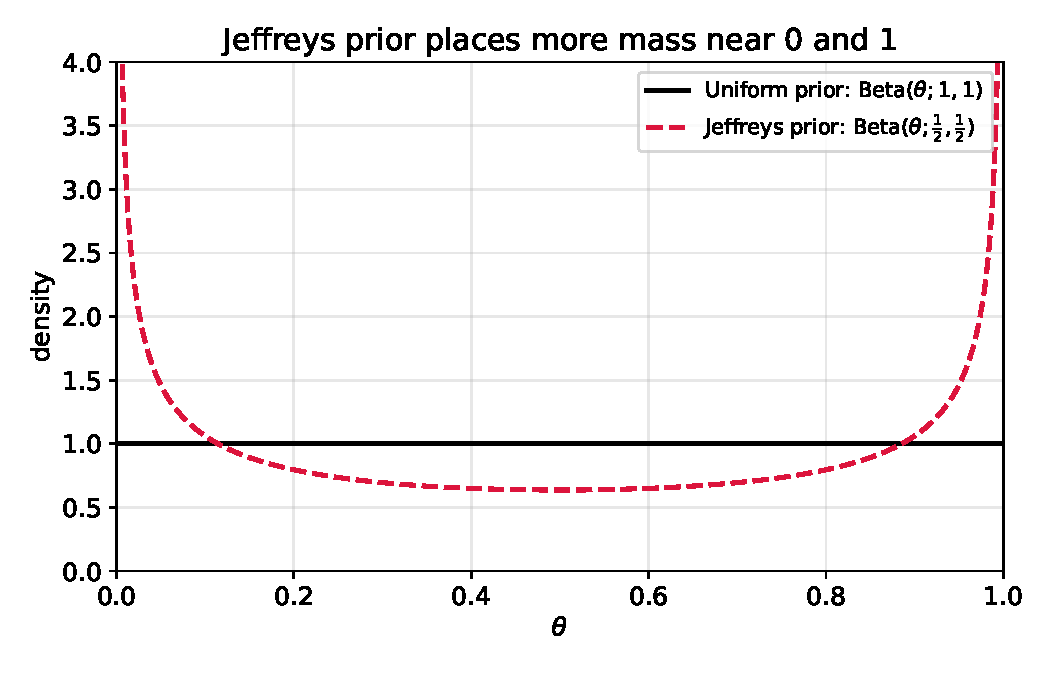
\includegraphics[width=\textwidth]{jeffreys_prior}
      \end{center}
    \end{column}
  \end{columns}
  As the figure shows, the Jeffreys/KT prior (dashed red) places
  \emph{more} density near the extremes $\theta=0,1$ than the flat uniform
  prior (solid black), reflecting the fact that a Beta$(\tfrac12,\tfrac12)$
  prior is slightly more open to a strongly biased coin than the
  indifference prior is.
\end{frame}

\begin{frame}[fragile]{Python: KT estimator vs.\ Laplace estimator}
  \begin{lstlisting}
def beta_predictive(sequence, alpha, beta):
    """P(next flip = 1 | sequence), general Beta(alpha,beta) prior, (2.4.10)."""
    n = len(sequence)
    b = sum(sequence)          # number of ones
    return (b + beta) / (n + alpha + beta)

seq = [0, 0, 1]  # x_{1:3} = 001, as in Figure 2.11 of the book

laplace_pred = beta_predictive(seq, alpha=1, beta=1)      # uniform prior
kt_pred      = beta_predictive(seq, alpha=0.5, beta=0.5)  # Jeffreys/KT prior

print(f"Laplace rule P(x4=1|001) = {laplace_pred:.4f}")  # 0.4000
print(f"KT estimator P(x4=1|001) = {kt_pred:.4f}")        # 0.3750

# Strong-fair-coin prior: alpha=beta=20 (pseudocounts of 20 heads, 20 tails)
fair_pred = beta_predictive(seq, alpha=20, beta=20)
print(f"Strong-fair-coin prior P(x4=1|001) = {fair_pred:.4f}")  # 0.4767
  \end{lstlisting}
  With only three observations, the strong ``fair-coin'' prior
  ($\alpha=\beta=20$) barely moves away from $\tfrac12$, while the KT and
  Laplace estimators react much more quickly to the data -- exactly the
  behaviour described by the concentration-parameter discussion below.
\end{frame}

\begin{frame}{Decomposition: Bayes estimator as a convex combination}
  Equation (2.4.10) admits a clean decomposition:
  \begin{block}{Decomposition and concentration (2.4.12)}
    \[
      \mathrm P(X_{n+1}=1\mid x_1,\ldots,x_n;\alpha,\beta) \;=\; \lambda\bar x+(1-\lambda)\left(\frac{\beta}{\alpha+\beta}\right),
      \qquad \lambda=\frac{n}{n+\alpha+\beta},\quad \bar x=\frac1n\sum_{i=1}^n x_i.
    \]
  \end{block}
  Every symbol: $\bar x$ (x-bar) is the plain relative frequency of ones --
  i.e.\ the MLE, based solely on the data with no prior knowledge; the term
  $\beta/(\alpha+\beta)$ is the \emph{mean of the prior}
  $\mathrm{Beta}(\theta;\alpha,\beta)$, i.e.\ the ``pure prior'' estimate
  returned when no data at all is available; and $\lambda\in[0,1]$ (lambda)
  is a mixing weight. So the Bayes predictive estimator is exactly a
  \textbf{convex combination of the MLE and the pure-prior estimate}. Since
  $\lambda\to 1$ as $n\to\infty$ (for fixed $\alpha,\beta$), the influence of
  the prior fades away as more data arrives -- and because $\alpha+\beta$
  controls how much weight the prior estimate retains for any fixed $n$,
  the quantity $\alpha+\beta$ is called the \emph{concentration parameter}.
\end{frame}

\begin{frame}{Posterior mean and variance: confidence in $\theta$}
  As for the posterior $\mathrm{Beta}(\theta;b+\alpha,a+\beta)$ itself, its
  mean and variance are
  \begin{block}{Posterior mean and variance (2.4.13)--(2.4.14)}
    \[
      \mathbf E[\theta\mid x_1,\ldots,x_n] \;=\; \frac{b+\beta}{n+\alpha+\beta},
      \qquad
      \mathbf{Var}[\theta\mid x_1,\ldots,x_n] \;=\; \frac{(a+\alpha)(b+\beta)}{(a+\alpha+b+\beta)^2(a+\alpha+b+\beta+1)}.
    \]
  \end{block}
  Every symbol: $a,b$ are again the number of zeros and ones observed; the
  mean is exactly the predictive probability derived above; and the
  variance shrinks as either the amount of data $n=a+b$ grows or the
  concentration $\alpha+\beta$ (i.e.\ prior strength) grows.

  \begin{block}{Take-away}
    The posterior has \emph{low variance} (hence \emph{high confidence} in
    $\theta$) whenever \textbf{at least one of $n$ or $\alpha+\beta$ is
    large}. For $\alpha+\beta\gg n$, the posterior concentrates around the
    prior belief $\beta/(\alpha+\beta)$; for $n\gg\alpha+\beta$, the
    posterior concentrates around the relative frequency $b/n$ of ones --
    matching the intuition that with enough real data, the data
    ``overrules'' whatever prior we started with.
  \end{block}
\end{frame}

% =======================================================================
\section{Summary}

\begin{frame}{Chapter 2.4 summary}
  \begin{itemize}
    \item \textbf{Bayes' theorem} (Theorem 2.4.2) turns a prior
      $\mathrm P(H_i)$ and a likelihood $\mathrm P(D\mid H_i)$ into a
      posterior $\mathrm P(H_i\mid D)$, normalised by the evidence
      $\mathrm P(D)$.
    \item Probability has (at least) four common interpretations --
      frequentist, objectivist, subjectivist, Bayesian -- which differ in
      \emph{meaning} but all obey the same Kolmogorov axioms.
    \item Treating an unknown parameter $\theta$ as a random variable with
      prior $w(\theta)$ lets us apply Bayes' rule to \emph{parameter
      estimation}: joint $p(x,\theta)$, mixture/evidence
      $p(x_1,\ldots,x_n)$, posterior $w(\theta\mid x_1,\ldots,x_n)$, and
      predictive distribution $p(x_{n+1}\mid x_1,\ldots,x_n)$.
    \item For i.i.d.\ Bernoulli data and a $\mathrm{Beta}(\alpha,\beta)$
      prior, the posterior stays Beta (a \emph{conjugate} family), and the
      predictive probability of the next $1$ is
      $(b+\beta)/(n+\alpha+\beta)$.
    \item $\alpha=\beta=1$ gives the classical \textbf{Laplace rule}
      $(k+1)/(n+2)$; $\alpha=\beta=\tfrac12$ (the \textbf{Jeffreys prior})
      gives the \textbf{KT estimator}, invariant under reparametrisation.
    \item The Bayes predictive estimator is always a \emph{convex
      combination} of the MLE and the pure-prior mean, with the
      \emph{concentration parameter} $\alpha+\beta$ controlling how fast
      the data overtakes the prior.
  \end{itemize}
  \vspace{0.2cm}
  \textbf{Looking ahead:} later chapters replace this simple parametric
  $\theta\in\Theta$ setting with a \emph{universal} prior over all
  computable measures (Solomonoff's prior, related to Kolmogorov
  complexity), extending exactly the same Bayesian machinery to build the
  AIXI agent.
\end{frame}

\end{document}
